%

\subsection{Twierdzenie Pitagorasa}
Najważniejszym twierdzeniem dotyczącym trójkątów prostokątnych jest twierdzenie Pitagorasa oraz twierdzenie do niego odwrotne.
Piszą o~nim Guzicki \cite[s. 160]{guzicki_2021}.

% TODO: https://en.wikipedia.org/wiki/Pythagorean_theorem liczne dowody, wiek Pitagorasa

\begin{theorem}[Pitagorasa]
\index{twierdzenie!Pitagorasa}%
\label{theorem_pythagorean}%
    Niech $ABC$ będzie trójkątem prostokątnym, w~którym kąt przy wierzchołku $C$ jest prosty.
    \begin{center}\begin{tikzpicture}[scale=.4]
        %\tkzInit[xmin=-0.5,xmax=6.5, ymin=-0.5,ymax=4.5]
        % \tkzClip
        \tkzDefPoint(0, 0){A}
        \tkzDefPoint(0, 5){B}
        \tkzDefPoint(-2.4, 1.8){C}
        \tkzDefPoint(-2.7, 1.6){CC}
        \tkzLabelPoint[below right](A){$A$}
        \tkzLabelPoint[above right](B){$B$}
        \tkzLabelPoint[left](CC){$C$}
        \tkzDefSquare(B,A)
        \tkzDrawPolygon[fill=black!50](B,A,tkzFirstPointResult, tkzSecondPointResult)
        \tkzDefSquare(C,B)
        \tkzDrawPolygon[fill=black!25](C,B,tkzFirstPointResult, tkzSecondPointResult)
        \tkzDefSquare(A,C)
        \tkzDrawPolygon[fill=black!25](A,C,tkzFirstPointResult, tkzSecondPointResult)
        \tkzDrawPolygon[line width=0.4mm](A,B,C)
    \end{tikzpicture}\end{center}
    Wtedy suma pól jasnych kwadratów jest równa polu ciemnego kwadratu:
    \begin{equation}
        |BC|^2 + |AC|^2 = |AB|^2.
    \end{equation}
    Odwrotnie, jeśli $ABC$ jest trójkątem takim, że $|BC|^2 + |AC|^2 = |AB|^2$, to trójkąt ten jest prostokątny, zaś kąt przy wierzchołku $C$ jest prosty.
\end{theorem}

Chociaż współcześnie powyższe twierdzenie przypisujemy Pitagorasowi z~Samos, to nie wiemy dokładnie, kto i~kiedy odkrył je jako pierwszy.
\index[persons]{Pitagoras z Samos}%
Było powszechnie stosowane w~okresie Starego Babilonu (XX-XVI wiek p.n.e.), a~więc na długo przed narodzinami Pitagorasa; pojawia się też w indyjskich i~chińskich tekstach matematycznych.
Papirus Berlin 6619 spisany ok. 1800 roku p.n.e. na terenach państwa egipskiego zawiera zadanie, którego rozwiązaniem jest trójka $(6, 8, 10)$.
Jest jeszcze babilońksa tabliczka Plimpton 322, także spisana ok. 1800 roku p.n.e., gdzie pojawia się trójka (12709, 13500, 18541), co sugeruje, że jej autor znał pewną systematyczną metodę.

Być może twierdzenie Pitagorasa ma więcej znanych dowodów niż jakiekolwiek inne (poza prawem wzajemności reszt kwadratowych), jest ich obecnie tak dużo, że nie wiadomo, ile dokładnie.
Niektóre opierają się na rozcięciu pewnej układanki na fragmenty, przestawieniu ich i zbudowaniu innego kształtu.
Inne korzystają z podobieństwa trójkątów.
Dowód Euklidesa korzysta z zasady Cavalieriego i urzekł nas tak bardzo swoją pomysłowością, że będzie jedynym, jaki przedstawimy w~całej książce!
\todofoot{Przerysować obrazek} % https://en.wikipedia.org/wiki/File:Illustration_to_Euclid%27s_proof_of_the_Pythagorean_theorem2.svg

\begin{proof}
    Niech $\triangle ACB$ będzie trójkątem prostokątnym, z kątem prostym przy wierzchołku $A$.
    Na bokach $BC$, $AB$, $CA$ kreślimy kolejno kwadraty $CBDE$, $BAGF$, $ACIH$ (konstrukcja kwadratu Euklidesa korzysta z postulatu równoległości).

    \begin{figure}
    \end{figure}
    Z punktu $A$ opuszczamy wysokość na przeciwprostokątną $BC$ i przedłużamy tak, by przecięła kwadrat $CBDE$ w punktach $K$ i $L$.
    Łączymy punkty $A$ i $D$ oraz $C$ i $F$.
    Otrzymane trójkąty $\triangle ABD$ oraz $\triangle FBC$ są przystające na mocy cechy bok-kąt-bok ($AB$, $\angle ABD$, $BD$ oraz $FB$, $\angle FBC$, $BC$).
    Prostokąt $BDLK$ (odpowiednio: kwadrat $BAGF$) ma dwukrotnie większe pole niż trójkąt $\triangle ABD$ (trójkąt $\triangle FBC$).
    Zatem prostokąt $BDLK$ i kwadrat $BAGF$ mają równe pola.
    
    Analogicznie pokazujemy, że prostokąt $CKLE$ i kwadrat $ACIH$ mają równe pola.
    Dodajemy dwie równości stronami i otrzymujemy, że suma pól kwadratów $ACIH$ oraz $BAGF$ jest równa polu kwadratu $BCDE$.
\end{proof}

Legenda głosi, że Hippazos z Metapontu został utopiony po odkryciu, że przeciwprostokątna trójkąta o~przyprostokątnych równej długości nie jest współmierna z nimi; zrujnował tak pogląd pitagorejskiej szkoły, że świat opiera się na liczbach (czyli liczbach naturalnych oraz ułamkach z~nich zbudowanych).
Jeśli tak było, doprowadziło to do rozłamu szkoły.

\begin{corollary}
    Długość przekątnej prostokąta o bokach długości $a$ i $b$ wynosi $\sqrt{a^2 + b^2}$.
\end{corollary}

Względnie pierwsze liczby naturalne $a, b, c$ takie, że $a^2 + b^2 = c^2$ nazywamy (pierwotną) trójką pitagorejską.
Każdą taką trójkę można otrzymać biorąc względnie pierwsze liczby $m, n$ różnej parzystości takie, że $m > n$ i kładąc $a = m^2 - n^2$, $b = 2 mn$, $c = m^2 + n^2$.
Najmniejszą taką trójką jest $(3, 4, 5)$; inna legenda (nie było w niej ani smoków, ani Hippazosa) głosi, że Egipcjanie używali tego trójkąta do wyznaczania kątów prostych u podstawy piramid.

\begin{proposition}
    % TODO: rysunek z Guzickiego, stron 160
    Mają miejsce następujące równości:
    \todofoot{Brakuje rysunku}
    \begin{equation}
        h = \frac{ab}{c}, \quad
        p = \frac{b^2}{c}, \quad
        q = \frac{a^2}{c}, \quad
        h^2 = pq.
    \end{equation}
\end{proposition}

Twierdzenie Pitagorasa znajduje zastosowanie także przy wyznaczaniu niektórych miejsc geometrycznych.

\begin{proposition}
    Dane są dwa różne punkty $A$ i $B$ na płaszczyźnie oraz liczba rzeczywista $c$ taka, że $2c > |AB|^2$.
    Miejscem geometrycznym punktów $P$ o własności $|AP|^2 + |BP|^2 = c$ jest okrąg o środku w środku odcinka $AB$ i promieniu $r = \frac 1 2 \sqrt{2c - |AB|^2}$.
\end{proposition}

\begin{proposition}
    Dane są dwa różne punkty $A$ i $B$ na płaszczyźnie oraz liczba rzeczywista $c$.
    Miejscem geometrycznym punktów $P$ o własności $|AP|^2 - |BP|^2 = c$ jest prosta prostopadła do prostej $AB$.
\end{proposition}

Patrz Guzicki \cite[s. 170-173]{guzicki_2021} (Guzicki wprowadza potem osie i środki potęgowe jak w~fakcie \ref{guzicki_6_11}, a następnie twierdzenie \ref{guzicki_6_13} (Carnota)).

\todofoot{Xuan tu, spirala Teodorusa, dowód Garfielda}
% https://en.wikipedia.org/wiki/Xuan_tu
% https://en.wikipedia.org/wiki/Spiral_of_Theodorus
% https://en.wikipedia.org/wiki/Garfield%27s_proof_of_the_Pythagorean_theorem